%
% File acl2021.tex
%
%% Based on the style files for EMNLP 2020, which were
%% Based on the style files for ACL 2020, which were
%% Based on the style files for ACL 2018, NAACL 2018/19, which were
%% Based on the style files for ACL-2015, with some improvements
%%  taken from the NAACL-2016 style
%% Based on the style files for ACL-2014, which were, in turn,
%% based on ACL-2013, ACL-2012, ACL-2011, ACL-2010, ACL-IJCNLP-2009,
%% EACL-2009, IJCNLP-2008...
%% Based on the style files for EACL 2006 by 
%%e.agirre@ehu.es or Sergi.Balari@uab.es
%% and that of ACL 08 by Joakim Nivre and Noah Smith

\documentclass[11pt,a4paper]{article}
\usepackage[hyperref]{acl2021}
\usepackage{times}
\usepackage{latexsym}
\usepackage{graphicx}
\usepackage{float}
\renewcommand{\UrlFont}{\ttfamily\small}

% This is not strictly necessary, and may be commented out,
% but it will improve the layout of the manuscript,
% and will typically save some space.
\usepackage{microtype}

%\aclfinalcopy % Uncomment this line for the final submission
%\def\aclpaperid{***} %  Enter the acl Paper ID here

%\setlength\titlebox{5cm}
% You can expand the titlebox if you need extra space
% to show all the authors. Please do not make the titlebox
% smaller than 5cm (the original size); we will check this
% in the camera-ready version and ask you to change it back.

\newcommand\BibTeX{B\textsc{ib}\TeX}

\title{Instructions for ACL-IJCNLP 2021 Proceedings}

\author{First Author \\
  Affiliation / Address line 1 \\
  Affiliation / Address line 2 \\
  Affiliation / Address line 3 \\
  \texttt{email@domain} \\\And
  Second Author \\
  Affiliation / Address line 1 \\
  Affiliation / Address line 2 \\
  Affiliation / Address line 3 \\
  \texttt{email@domain} \\}

\date{}

\begin{document}
\maketitle
\begin{abstract}
This is the report of the project for the Web Recommender System course held at the University of Copenhagen.
\end{abstract}

\section{Week 6 [Feb 3 - Feb 9]: Familiarize Yourself with the Datasets}

\subsection{Dataset Description and Import}
The dataset used in this project is the ``Musical Instruments'' dataset from the Amazon Review data 2023 (5-core subset). The dataset consists of 14,000 item ratings from nearly 900 users on approximately 500 items. The data is split into training and test sets, with 80\% of the data allocated for training (``train.tsv'') and 20\% for testing (``test.tsv'').

The dataset was imported using the Python library \texttt{pandas}\cite{pandas} and its \texttt{read\_csv} function.

\subsection{Data Cleaning and Preprocessing}
To ensure the quality of the dataset, we performed the following preprocessing steps:

\begin{itemize}
    \item Removal of missing values (entries with missing user ID, item ID, or rating).
    \item Deduplication by keeping the most recent rating when a user rated the same item multiple times.
    \item Ensuring that all users in the test set are also present in the training set.
\end{itemize}

In terms of dimensions the effect of the cleaning can be summarized in the \autoref{tab:cleaning_effect}.

\begin{table}[H]
    \centering
    \resizebox{1\columnwidth}{!}{
    \begin{tabular}{lll}
    \textbf{Dataset} & \textbf{Before Cleaning} & \textbf{After Cleaning} \\
    Train Set & 11000 & 9913 \\
    Test Set & 3000 & 1822 \\
    \end{tabular}
    }
    \caption{Effect of the Data Cleaning Process}
    \label{tab:cleaning_effect}
    \end{table}

\subsection{Exploratory Data Analysis (EDA) and Statistics}
To gain insights into the dataset, we computed the following statistics:

\begin{itemize}
    \item Distribution of ratings per user in \autoref{fig:ratings_per_user}
    \item Distribution of ratings per item in \autoref{fig:ratings_per_item}
    \item Overall rating value distribution in \autoref{fig:rating_value_distribution}
\end{itemize}

\begin{figure}[H]
    \centering
    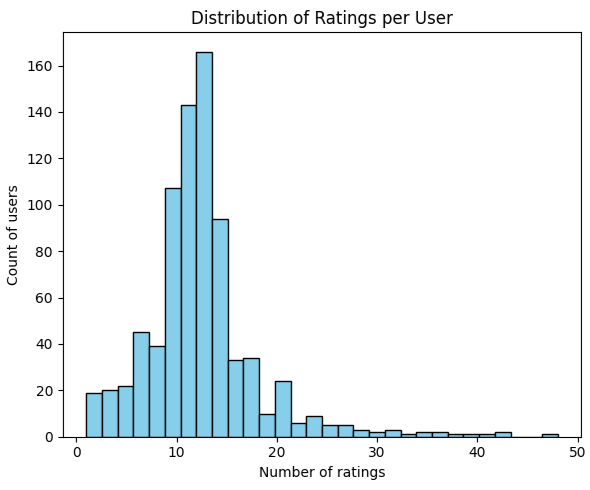
\includegraphics[width=0.8\columnwidth]{Images/ratings_per_user.png}
    \caption{Distribution of Ratings per User}
    \label{fig:ratings_per_user}
\end{figure}

\begin{figure}[H]
    \centering
    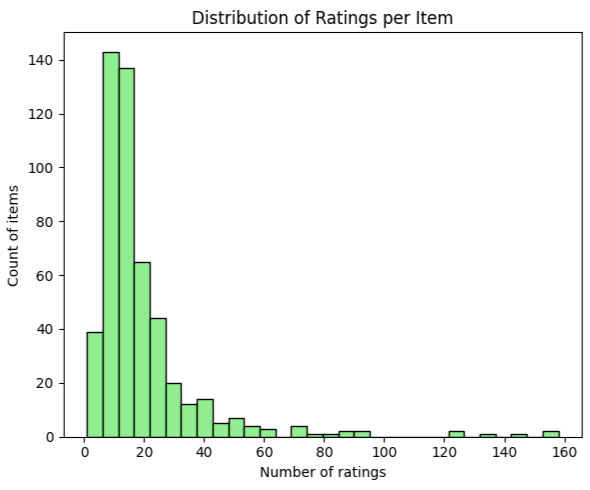
\includegraphics[width=0.8\columnwidth]{Images/ratings_per_item.png}
    \caption{Distribution of Ratings per Item}
    \label{fig:ratings_per_item}
\end{figure}

\begin{figure}[H]
    \centering
    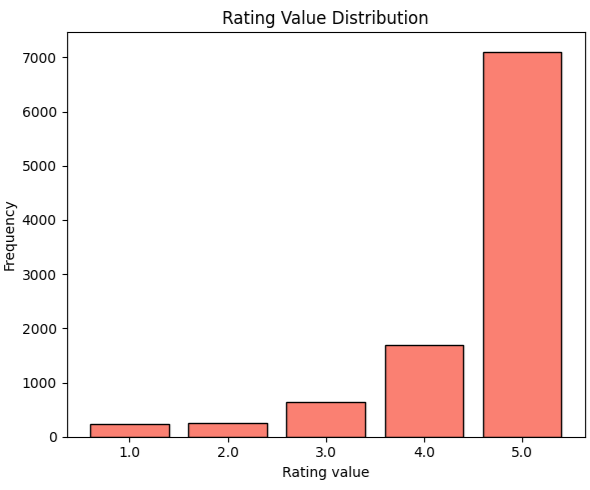
\includegraphics[width=0.8\columnwidth]{Images/rating_value_distribution.png}
    \caption{Distribution of Ratings per Vlaue}
    \label{fig:rating_value_distribution}
\end{figure}

Also, to show the long-tail distribution of ratings, we plotted the number of ratings per item in \autoref{fig:long_tail}.

\begin{figure}[H]
    \centering
    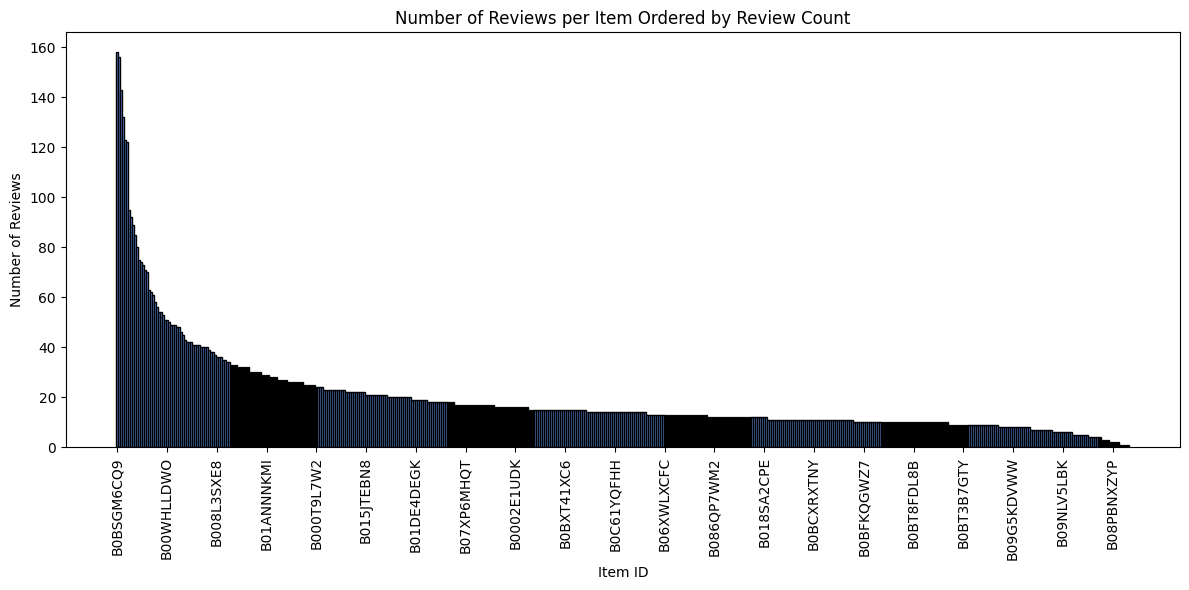
\includegraphics[width=1\columnwidth]{Images/long_tail.png}
    \caption{Long tail distribution of rating over all the items}
    \label{fig:long_tail}
\end{figure}

\subsection{Highly Rated Items}
To identify popular items, we computed the number of ratings \(\geq 3\) for each item and reported the top 5 most highly rated items in \autoref{tab:top5_items}.

\begin{table}[H]
\centering
\resizebox{1\columnwidth}{!}{
\begin{tabular}{lll}
\textbf{Item ID} & \textbf{High Ratings Count} & \textbf{Average High Rating} \\
B0BSGM6CQ9 & 153 & 4.784 \\
B0BPJ4Q6FJ & 153 & 4.804 \\
B09857JRP2 & 141 & 4.809 \\
B0BCK6L7S5 & 120 & 4.583 \\
B0BTC9YJ2W & 119 & 4.815 \\
\end{tabular}
}
\caption{Top 5 Most Highly Rated Items}
\label{tab:top5_items}
\end{table}

\subsection{Discussion}
The dataset exhibits common characteristics of user-item interactions:

\begin{itemize}
    \item There is a long-tail distribution where a small number of items receive most of the ratings, while many items have very few ratings.
    \item The majority of users have rated only a few items, which can lead to sparsity issues in collaborative filtering approaches.
    \item Certain items dominate the high-rated category, which may bias recommendation systems.
\end{itemize}

\bibliographystyle{acl_natbib}
\bibliography{acl2021}

%\appendix



\end{document}
